

\documentclass{article}% use option titlepage to get the title on a page of its own.

\linespread{1.4}

\usepackage{lmodern}
\usepackage{listings}
\usepackage{color}

\definecolor{dkgreen}{rgb}{0,0.6,0}
\definecolor{gray}{rgb}{0.5,0.5,0.5}
\definecolor{mauve}{rgb}{0.58,0,0.82}

\usepackage{graphicx}
\graphicspath{ {./images/} }



\title{%
  Political Manifesto Analysis \\
  \large Technical Report}

\date{2019, January}
\author{Giovanni Misseri, Mohammad Kameli, Jolan Chabbey \\ \\ 
Network Science course}
\begin{document}
\maketitle
\section{Introduction}
In this relation we will try to explain and justify what we've done in order to analyze the european political society.
As one can imagine the political world is dense of alleances, sometimes decleared and sometimes unspoken; and even a bigger problem is the one of understanding the actual political thought of a party.
Usually each party declears itself as lined up on right center or left side, but in practice often it's really hard to define what makes a party a right side or left side party and if we just look at how a certain party acts the definition becomes even more fuzzy.\\

What we aim to achieve with this work is to derive and analize the network of european parties in a cross-temporal analysis. As we said is not always the case that a party that declares itself as a left side party, acts like a left side party. Due to this reason to construct the network in which each party is a node, we will link two parties not if they declare to collaborate each other and nor if they have some political alleance, we will try to link two nodes if the two connected parties have the same idea on some critical concepts.\\

On such network we will run our analysis trying to spot behaviours and insits of the political scene. Moreover we will try to detect the communities inside this network in order to see if the actual division of the parties overlaps with the decleared one, and consequently see which are the parties that, based on their ideas, are not distiguishable by their adversary.

\section*{Manifesto Project}

The Manifesto Project - "https://manifesto-project.wzb.eu/" - is a German project which aims to mantain and contiously update different political dataset. Their main work is the "Manifesto Project Dataset", a dataset containing at the moment 4388 political manifestos published from 1945 till today by 1117 parties.
They publish and mantain this dataset in order to be able to conduct scientific research on the european political field, but not explicitly exploiting network science or graph theory.

We found this project really interesting because contains information about the processing of parties' the political manifestos. The great advantage of using the Manifesto Project work is not only the high number of manifestos present there, but also 
the way they extracted information about manifestos and how they ecoded that.
In Manifesto Project dataset there is a good number of variables representing diferent ideas, like "Imperialism" or "Welfare State Expansion", giving tham for each manifesto a score representing "how much a manifesto reflects that idea".
\\

As we said we wanted to build a network of parties exploiting what they think and not what they declare, here the limit is evident but building a network on political manifesto and the ideas that it reflects could be considered a good approximation of reality.

We will than exploit Manifesto Project dataset to build our network.
\\
\\
\\


\section{The Network}

The first problem we had to deal with is how to exploit a general dataset to build a meaningfull network. We come up with a nice idea and after some research we found out that it's a quite used way to proced. 
Before talking about how we built our adjacncy matrix it's important to underlign the data engeneering we went through.

Our dataset was composed by 1117 parties and we had in total 4388 manifestos, so we had an avererage of 4 manifestos for each party. We had to decide how to deal with the greater number of manifestos with respect to the parties. A natural way to proceed is to average the score of the manifestos for each party, and that's what we did. This is a meaningfull way to proceed because like that what we work on is an averege idea's score over the time for each party. Another possible way to proceed would be taking only the last available manifesto's score, one would have obtained the most recent data but losing past information, this could bring to biased masures due to the variability of ideas in parties, a mean over time brings to zero the score for all that ideas where a party showed contradictorial positions over time, underlining the one where a party actualy based his existnce.
\\

Said that we can jump to the adjacency matrix. We took our restructured dataset made by 1114 rows, the number of parties without missing data in taget variables, and 56 coulmns, the set of main ideas Manifesto Project gives score. First of all we computed the paiwise distance matrix, in which in position \emph{i,j} is present the euclidean distance between party's \emph{i} ideas and party's \emph{j} ideas. 
At this point we needed to decide a treshold for which if two parties are nearer than that, they are connected, otherwise theey are not. This approach will create a simmetric unwheighted adjacency matrix and will be the one on which we will conduct the gratest part of our analysis.
A particularity of this approach is that is comparable with the hierarchical clustering in particular with the sigle linkage hierarchical clustering, this will be crucial for future analysis.
We decided to cut the distance matrix at 10. We choose this value on further analysis and this is the treshold that created the most reasonable matrix. With a higher value we would have had more connected nodes, but on the other hand we would have lost important links; with a lower value we would have had too muchnodes not connected with no other node.

\section*{Preliminary Analysis}

After the $\epsilon$-neighborhood procedure explained before to create the adjacency matrix we are ready to do some analysis on our graph. First of all we start with some preliminary analysis in order to understand the context we are working on and the kind of graph we have to deal with.
\\

As first importand step is necessary to remove all the nodes that are not connected at all, since we can't gain more information from their inclusion in futher analysis. Anyway given the fact that we have 549 nodes that are not connected at all this is an important limit to our analysis, so it's important to understand why almost half of the nodes are not connected with no other node. Generally it's normal the presence of some outlier in your dataset when you compute your analysis,  but here we have a significant part of our data showing this behaviour. A possible interpretation could come from the context the data come from; we are talking about parties and what they put in their manifestos, saying that two parties are connected only if they are sufficiently near implyes that we cut all that links that exist on the "margin" of our network, we will take only the central part of the network. This seems confirmed also by the political interpretation one can give to this phenomenon, with this approach we are able to correctly catch the relations between "central" parties, but we exclude all the extreme parties.
Don't forget also that our dataset ranges from 1945 till now, so seems reasonable that there was lot of different parties, not necessary extreme in the political meaning but very different one from the others.

An other mathematical reason could be due to the way we built our adjacency matrix. Apart from the treshold we had to decide, the quantity of single nodes could also due to the single linkage hierarchical clustering behaviour we talked before. 
\\

We that procedet to the delition of the single nodes and we obtaind a graph made by 656 nodes.
What follows is the related adjacecy matrix.

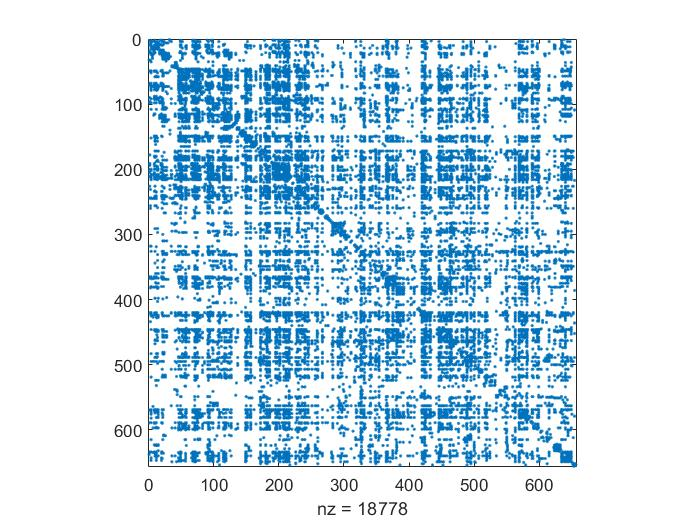
\includegraphics[scale=0.5]{Adj}

\section*{Nodes Distribution}

The first important aspect we what to inspect about the notwork is its degree destribution and its estimate. Moments of the degree distribution are of particular interest, in our case we have a network in which the avrage number of link for each node is 28.625, the variance is 1500.079 and the skewness is 1.7576.
So every party is connected on average to 28 other parties, but it's important to notice that, as we expected, we have a highly skewed degree distribution, sign of possible right outlier, alias hubs.


Let's inspect deeper this aspect through the probability distribution function and the log-pdf.

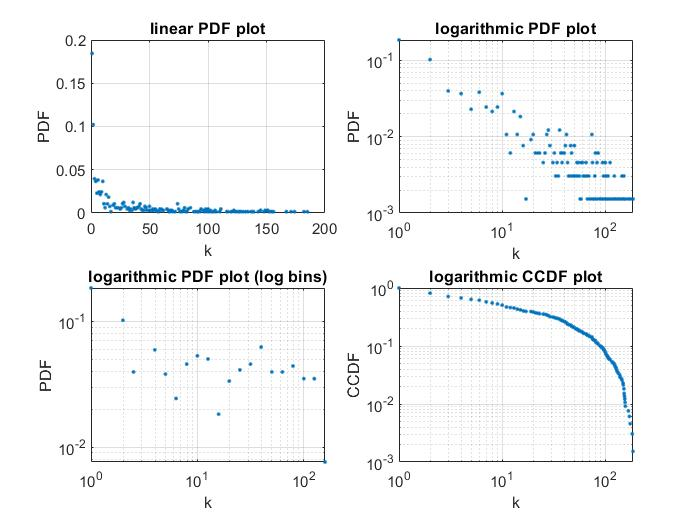
\includegraphics[scale=0.5]{Degree_distr}
\\

From the plots above is evident that as we supposed our network shows different features that makes it possibly a scale free network. For example we have clearly the grates part of nodes which have low degree and few points with high degree. The presence of hubs, indeed, is what distinguish a scale free network from a poisson distributed or random one. In this case the interpretation is a bit controversial, we have some nodes with high degree, but they don't follow the tipical linear decay in log-ccdf plot. 

One explanation for this phenomenon comes from log-pdf plot, from there we can see the linear decay, but it seems to have high variance. Given that this are real data we can't expect to find the well distributed probability distribution function and a linear decay with big variance justify our supposition of scale free distribution of our network.
Another way to justify tihs behavior comes again from the interpretation of our network in its context. We have parties connected one to the other, and would be unreasonable to have much parties connect with a lot of other parties. It would mean that we have some parties which ideas are similar to both right and left parties, we have some parties that are similar to a lot of other parties; as one can see this is not reasonable in this context. So we have some structural limit due to the context that doesn't allow our network to show a complete and satisfactory scale free behaviour.
\\

So with the underligned limits we will proceed the analysis assuming we are dealing with a scale free network with an high cut-off, so next step is to estimate the $\gamma$ parameter of the distribution.\\


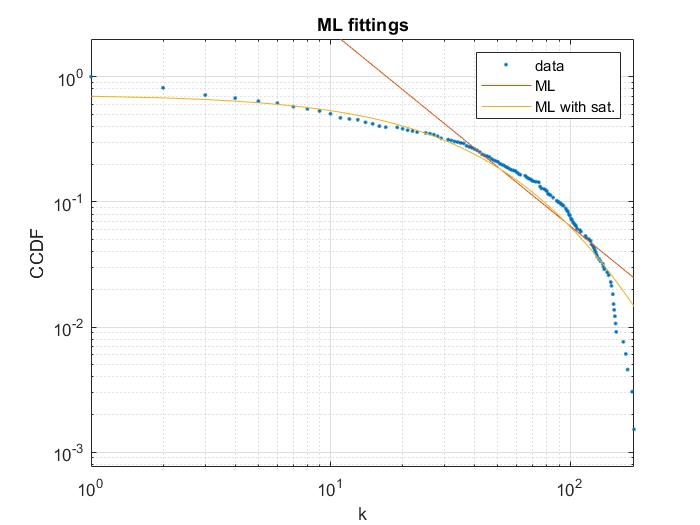
\includegraphics[scale=0.5]{ML_fit}
\\

The one reported above is the plot obtained by the estimation of the $\gamma$ exponent of the power low distribution of our network. The $\gamma$ parameter has been estimated using maximum likelihood, red line, and seems to approximate the log-ccdf behaviour. As we already said is strong the cut-off but the estimate of the $\gamma$ exponent with $k_{sat}$ approximate the ccdf quite well. 

The point estimate are respectively $2.5565$ and $6.6197$ for maximum likelihood estimate and ML with sat parameter. The high value obtained in the second case is due to the high cut-off present in the distribution, so we will consider the ML point estimate as $\gamma$ exponent of our power law distribution. 
As one can notice our power low exponent is between 2 and 3 so as we said we are in scale free regime with ultra small world property. A quite surprising property this one in our context, infact we would have extected to find a kind of compartimental network, in which nodes distribute in communities dense of link within their self but low connected between each other, this would have limited the ultra small world property instead this prooves that in realy few jumps we can go from extreme right nodes to extreme left nodes. This suggest an underlying homogeneity between parties that actualy seems to differ that low one from each other to result in an ultra small world regime.

\section*{Network Analysis}

In this chapter we would like to analyze different features of our network namely: Assortativity, Clustering coefficient, Robustness of the network to the random failure and an attack and finally find the communities in our network with different approaches.

\subsection*{Assortativity}

In general, (dis)assortativity stands for the preference of a network's nodes to attach to others due to their degree. In short, Assortative network is defined as high degree nodes connect with each other avoiding low degree nodes (tend to cliques) and Disassortative network tends to opposite trend, which means that hubs tend to avoid each other. 

For the political manifesto network, we expect to find the assortativity in our network regarding the parties with the same manifest tend to connect to each other though the hubs which may stand as the leader of right-left parties should avoid each other, thus not a perfect assortativity behavior but neither disassortative nor neutral network. Fig. 4 shows the assortativity of our network.
\\

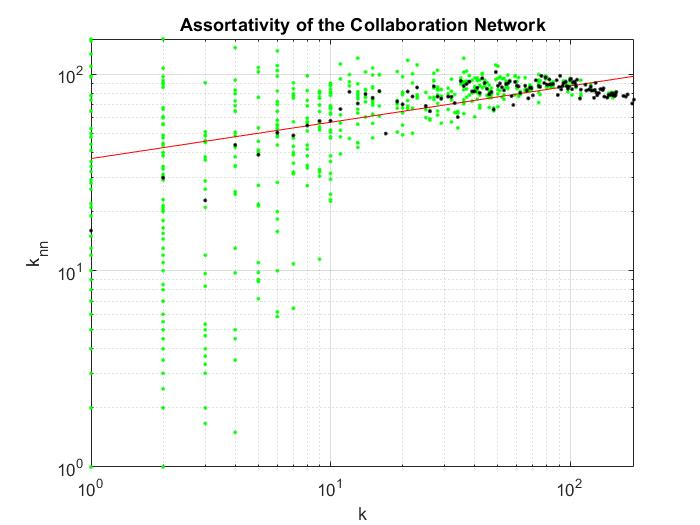
\includegraphics[scale=0.5]{Assortativity}
\begin{center}
\begin{small}
Fig. 4. Assortativity behavior of our network and fitting line for assortativity factor
\end{small}
\end{center}

~
\\

In this regard, we explore an assortative behavior as we expected and also a structural cut-off for k = 100. Finally the Assortativity factor is 0.18504 for our network.

An interpretation of the assortativity in this context suggest we are in the right direction and the positive assortativity estimation is supported too. If we carefuly think to what assortativity is and try to apply it to this context we will find that an assortative network is what we expected. Indeed given that the assortativity mesures "how mutch" hubs clusters with each other and how mutch low degree nodes do the same, we can translate this like a mesure of how mutch central parties tends to cluster and how mutch extreme parties tend to cluster. This phenomenon is then absolutely expected, would we weird infact to mesure disassortativity here, minor or extreme parties usualy are not directly connected with big parties, infact if their ideas were "the popular one" they wouldn't be minorities.

\subsection*{Clustering Coefficient}

Analyzing the neighbors of each parties lead us to find the clustering coefficient and compute the average clustering coefficient for political manifest network. In short, the clustering coefficient measures the density of links in the neighborhood which means how the parties which are tightened to each other as a neighbor are linked. Moreover, we plot the CCDF of the clustering coefficient to represent the behavior of the network for neighbors. Fig. 5. Show the result.
\\



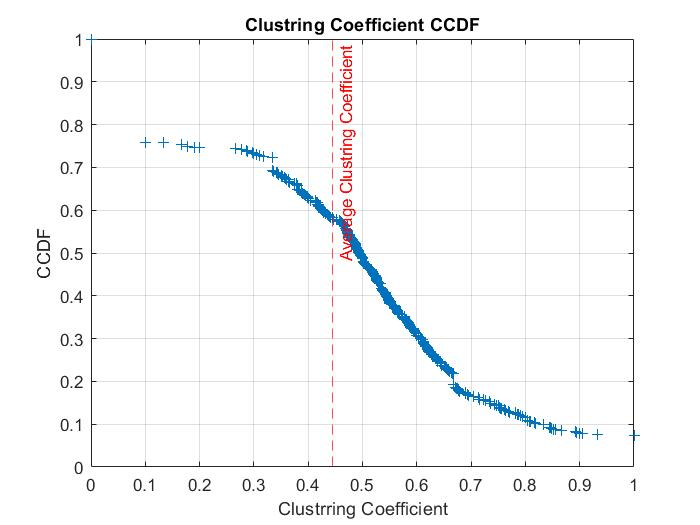
\includegraphics[scale=0.5]{Clustering_Coefficient}
\begin{center}
\begin{small}
Fig. 5. CCDF of clustering coefficient and average measurement
\end{small}
\end{center}

~
\\

In this figure we also consider the nodes which have zero coefficient which are almost 20\% of our nodes, due to that there parties which are not linked as a tripled graph. In addition, the average clustering coefficient measurement for our network is: 0.446.


\subsection*{Robustness}

One of the most important aspect of studying political manifest would be to find the robustness of the network. It leads us to find the property of being strong in a community.

Interesting part of this study would be to find when we can failure a network and how to do it. For instance, consider a competition that the right parties want to win the left parties. Utilizing this property each community could determine by enlisting which parties or ideas could lead the other community to collapse. Implementing robustness with attack could be consider as a future study of this network. 
\\

In our computational aspects we only consider whole network for random failure and an attack by removing random nodes and hubs with the highest degree respectively. Fig. 6 show the robustness of our network and as we could realize from the fig. 6. The distance between random failure and an attack for general network is robust and strong to attacks. Moreover, Molly-Reed criteria which is considered as a threshold for vanishing the giant component (GC) in our network is showed by a red line. It means network lower than that criteria would lose the GC.
\\


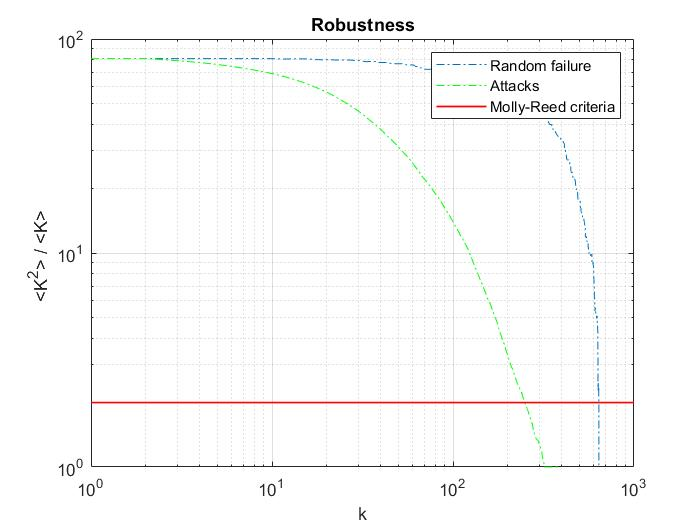
\includegraphics[scale=0.5]{Robustness}
\begin{center}
\begin{small}
Fig. 6. Robustness of the network for random failure (green) and attack (blue) with Molly-Reed criteria (red)
\end{small}
\end{center}

\section*{Community detection}

In this chapter we will talk about community detection and we will describe our steps to spot the communities in the manifesto network.

Our first idea was simply to go streight on with community detection on the usual adjacency matrix, but this resulted a bad approch for different reason.
We builted our matrix using an $\epsilon$-neighbour thecnique, as we said this is conceptually similal with respect doing hierarchical clustering using single linkage. Below a figure of a tipical a single linkage dendrogram.
In this example the blue line indicates where we decided to cut and the dot represent the connected component we get.

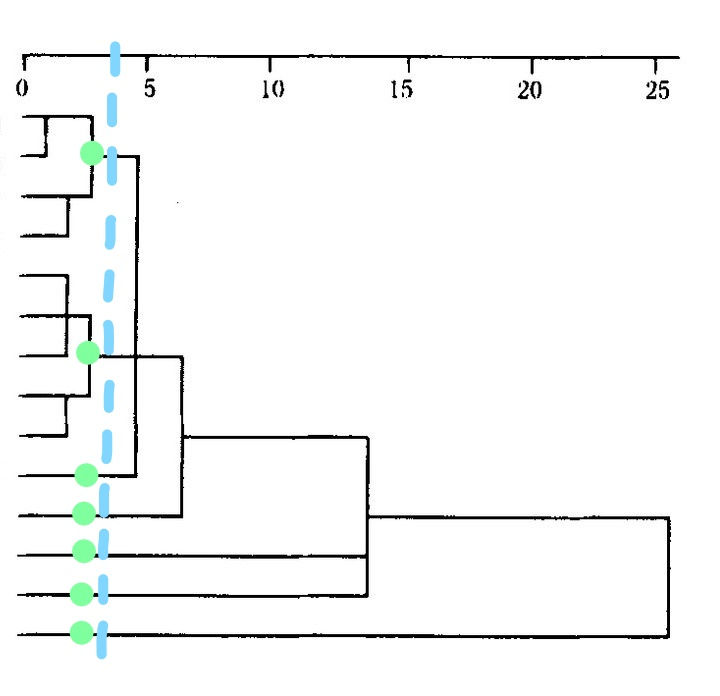
\includegraphics[scale=0.5]{Dendrogramma}
\begin{center}
\begin{small}
Fig. 7. Example of a single linkage dendrogram
\end{small}
\end{center}

~
\\

If we carefully think about what we did we discover that actually is the same think, we computed a distance matrix and we putted to 1 all the entries where we found a value less than $\epsilon$, 0 otherwise. Take it like a scratch of the proof by induction: at distance zero all nodes are disconnected, at distance one suppose two nodes link together, at distance 2 all the nodes nearer that 2 to a node belonging to this cluster will join too.

We end up in the situation shown in Fig 7. and actually is what happened to our network, indeed our network if made by different disconnected networks. Note also that this explain why we had that much nodes not connected to any other nodes, this is infact a common behaviour in single linkage hierarchical clustering, such that the presence of a biggest component.

Actually the disconnected components of our network already are a clustering, but our main aim is to divide the network in its natural tree communities: right, left and center.
The actual clustering naturally provided by disconnected components of the network doest provide such division.


The one below is a plot of our network.


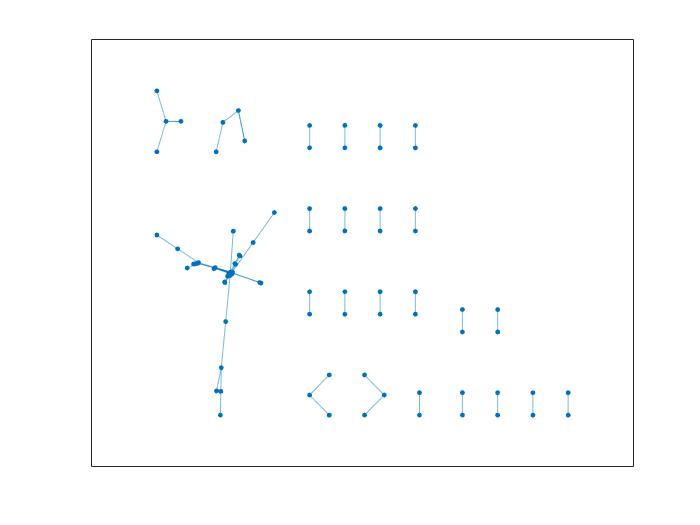
\includegraphics[scale=0.5]{disc_graph}
\begin{center}
\begin{small}
Fig. 8. Manifesto's network
\end{small}
\end{center}
~
\\

As shown in the figure our actual network doesn't fit the task of computing communities, and also doing clustering on the biggest component brought not satisfactory results.

We decided than to use a different approach and starting agin from the initial dataset, create a different adjacency matrix.
\\

Given that the gratest part of our problems come from th fact that our network was disconnected we worked to overcome that issue. We decided to use the distance matrix in order to build a Gaussian similarity matrix.
\\

So we set $Sim_{i,j}= exp(- \frac{||x_i-x_j||^2}{2\sigma^2})$ with $\sigma^2=200$. So we used this similarity matrix as adjacency matrix. We ended up with a full weighted graph and we run community detection algorithm on this.

We tried different approaches but given that we wanted a specific kind of communities we decided to rely on spectral approach. Theory sais infact that the minimum ratio-cut is the same problem of finding the minimum of finding the minimum of the Rylenght quotien, $\frac{(f'Lf)}{(f'f)}$, given some specific $f$ vector. The linear relaxation of this problem end up in finding the eigenvalues of the laplacian matrix of the network.

Not surprisingly is possible to proove that also the conductance is well approximated by the eigenvectors of the laplacian.
\\

We decided than to follow this path and we clustered our network in three communities, using kmeans algorithm on the nodes in the space of the last 3 eigenvectors. After some run of the algorithm we can say that if usualy converges to 3 communities respectively containing 755, 295 and 64 nodes.
\\

Below we report the sihlouette plot relative to our communities detection. Sihlouette is a mesure of how distant each point is from its cluster controid, so the higher the sihlouette value the more reliable the clustering is.

In our case we have a really good result for the bigger community and the smallest one, some doubts could come from the middle-size community for which some entry has low sihlouette value. Anyway this result plus the fact that kmeans converges almost everytime to the same communitis guarantee us these are reliable communities.

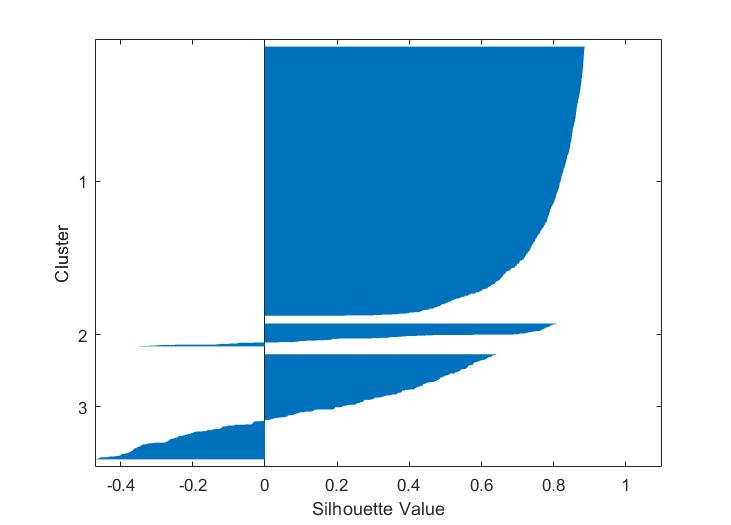
\includegraphics[scale=0.5]{sihlouette}
\begin{center}
\begin{small}
Fig. 9. Communities sihlouette
\end{small}
\end{center}
~
\\

Suggestion for further development of this analysis would be understan why we end up with these communities from a political point of view. 
In general we can say that on average manually computed communities and the kmeans overlaps on average on $45\%$ of parties.
\\

As we just said we also have a sort of classification provided by Manifesto project. Indeed they suggest a metric to discriminate right and left side parties, they attached a variable to the dataset meaning that. "Rile", the nominated variable, is defined as $ (per104 + per201 + per203 + per305 + per401 + per402 + per407 +
per414 + per505 + per601 + per603 + per605 + per606)
- (per103 + per105 + per106 + per107 + per403 + per404 + per406
+ per412 + per413 + per504 + per506 + per701 + per202) $ where $"per-"$ stends for the ID of an idea. For completness and to be able to "translate" the variable encoding we allegate also the Manifesto project codebook.


\section*{Ranking}

\subsection*{Page Rank}

\subsection*{Communicability}

In PageRank the importance of a node$i$  is proportional to the sum of the importances of the nodes $j$ pointing to it. This ceates a rank of nodes based on their importance in the network; but let us suppose now we want to assign to each node a number that quantifies its "well-connectedeness".

A natural choise would be $d_i^{in}= \sum_{j=1}^n A_{i,j}$ or $d_i^{out}= \sum_{i=1}^n A_{i,j}$, but the in degree and the out degree of a node paints a very localized picture of the overall well-connectedeness since they do not distinguish between edges that connect well connected or poorly connected nodes.
\[ (A^{2})_{ii}= \sum_{k=1}^n a_{i,k}a_{k,i}~~\rightarrow~~
(A^{k})_{ii}= \sum_{k=1}^n a_{i,k}a_{k,i}^k
\]

Where $(A^{k})_{ii}$ is the number of walks from $i$ to $i$ of length k. The idea is that a well connected node should have more opportunities to form a closed walk of small length. 
Shorter walks are tipically more important than longer walks, so we need to penalize the number of walks of length $k$, we choose as penalizing factor $\frac{1}{k!}$
\[ (I+A+\frac{A^2}{2!}+ ...+\frac{A^k}{k!}+...) =:e^A
\]
So we can define the subgraph centrality of the $i$-th node as $(e^A)_{ii}$. In general computing individual entries of a matrix function, in this case $f(A)=e^A$ is costly for large matrices. Anyway in recent years efficient algorithm have been developed for computing the action of a matrix function on a vector.
\\

Exploiting this last fact we can define the total comunicability of a node $i$ in a network defined by adjacency matrix A as
\[ t_i:=(e^{A^t}1)_i=\sum_{j=1}^n (e^{A^t})_{i,j}
\]
Where $t_i$ counts the number of walks between node $i$ and all the nodes in the network, weighting walks of length $k$ by a penalty factor of $\frac{1}{k!}$.


We can also obtain a mesure of total communicability of a network summing up all $t_i$ of each node.
\\

Said that we report below the communicability rank of our network.
\\

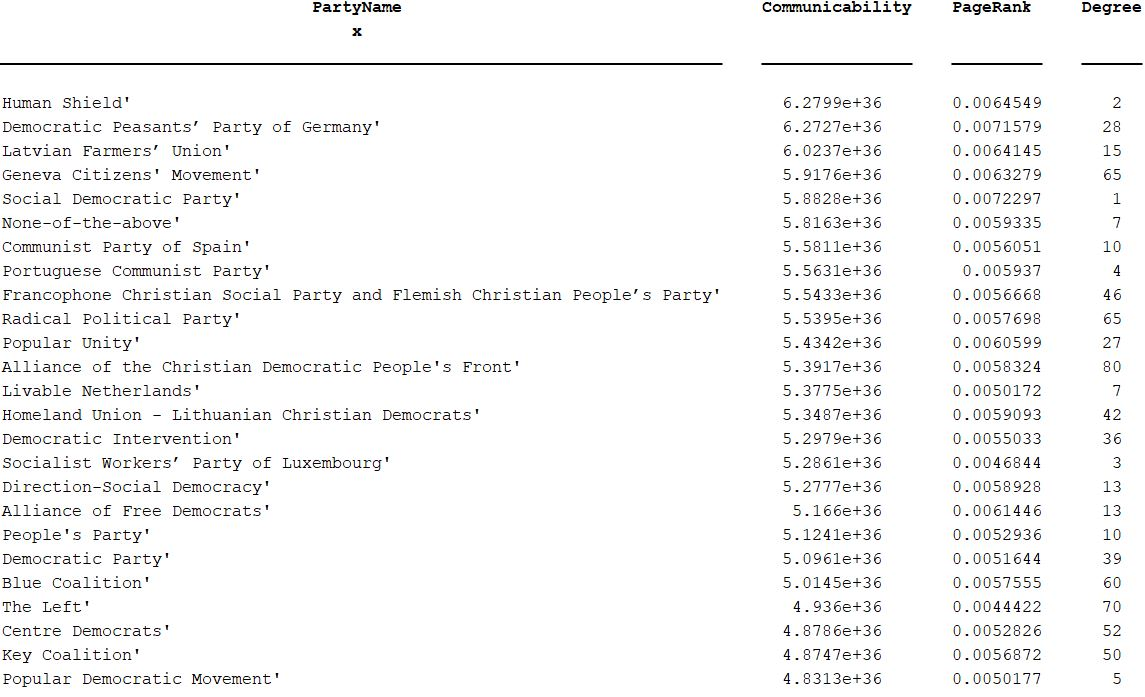
\includegraphics[scale=0.6]{communicability}
\begin{center}
\begin{small}
Fig. ---. Communicability rank 
\end{small}
\end{center}
~
\\
As one can notice PageRank and Communicability agrees on which are the most important nodes, but their ranking is not the same, there is some correlation between the two.
For further analysis would be interesting to see the robustness of the network if instead of attaking the hubs we attack each time the node with higher communicability. Also inspect why this partis results foundamental for communication.
To conclude there is one last really intersting application that could be taken into consideration for futher analysis, maybe also the most natural one, simulate the spreading on the network starting from high communicability nodes and mesure the effectiveness of the approach with respect to random start or hubs start.



\end{document}